\documentclass[aspectratio=43]{beamer}
\usepackage[latin1]{inputenc}
\usepackage{amsmath}
\usepackage{amsfonts}
\usepackage{amssymb}
\usepackage{makeidx}
\usepackage{graphicx}
\usepackage{array}

% Customization
\mode<presentation>{
	\usetheme{CambridgeUS}
	\usecolortheme{dolphin}
	\setbeamertemplate{navigation symbols}{}
}

% Define colors
\definecolor{darkgreen}{rgb}{0.0, 0.5, 0.13}
\definecolor{darkblue}{rgb}{0.0, 0.0, 0.55}
\definecolor{darkred}{rgb}{0.55, 0.0, 0.0}

% Title and author
\title[Introduction to statistics]{Introduction to statistics}
\author{\textbf {Jes\'us Urtasun Elizari}}
%\institute{\textbf {University of Milan}}
\date{London, April 2022}

\begin{document}

% Front slide
\begin{frame}

	%\maketitle
	\vspace{1.0 cm}
	
	\center{\color{blue}Introduction to statistics}
	
	\vspace{0.25 cm}
	\center{Computational biology week - London, April 2022}
	\center{Jes\'us Urtasun Elizari, PhD}
	
	\begin{figure}
		\minipage{1\textwidth}
		
\includegraphics[width = 3.0 cm]{plots/front_page/mrc.png}
		\hfill
		
\includegraphics[width = 3.0 cm]{plots/front_page/lms.png}
		\hfill
		
\includegraphics[width = 3.0 cm]{plots/front_page/icl.png}
		\endminipage
	\end{figure}

\end{frame}

% Introduction
\begin{frame}

	\frametitle{Outline}
	
	\begin{enumerate}
		\item {\color{blue}Probability in a nutshell}
		\begin{itemize}
			\item Discrete and continuous probability
			\item Mean and variance of a distribution
			\item Exercises in R
		\end{itemize}
		\item {\color{blue}Linear models}
		\begin{itemize}
			\item What is a linear model
			\item Fitting a linear model
			\item Prediction vs inference
			\item Exercises in R
		\end{itemize}
		\item {\color{blue}Hypothesis testing}
		\begin{itemize}
			\item Probability distributions
			\item Statistical tests
			\item Real genetics problem
			\item Exercises in R
		\end{itemize}
	\end{enumerate}
	
\end{frame}

%
% Probability in a nutshell ..............................................................
%

% Probability in a nutshell
\begin{frame}

	\center{\color{blue}Chapter I \\ Probability in a nutshell}

\end{frame}

% Probability in a nutshell
\begin{frame}

	\frametitle{Probability in a nutshell}
	\framesubtitle{Discrete and continuous probability}
	
	\footnotesize
	
	\begin{itemize}
		\item Discrete output $\longrightarrow$ probability well defined, compute by counting
		\item Continuous output $\longrightarrow$ need for probability distributions
		\item Definition of probability in both scenarios
		\item Computing probabilities in both scenarios
	\end{itemize}

\end{frame}

% Probability in a nutshell
\begin{frame}

	\frametitle{Probability in a nutshell}
	\framesubtitle{Discrete probability}
	
	\footnotesize
	
	Compute probability of getting 4 heads in a row

\end{frame}

% Probability in a nutshell
\begin{frame}
	
	\frametitle{Probability in a nutshell}
	\framesubtitle{Discrete probability}
	
	\footnotesize
	
	Compute probability of getting a specific genotype

\end{frame}

% Probability in a nutshell
\begin{frame}
	
	\frametitle{Probability in a nutshell}
	\framesubtitle{Binomial distribution}
	
	\footnotesize
	
	\begin{columns}	
		
		\column{0.5\textwidth}
		
		\begin{figure}
			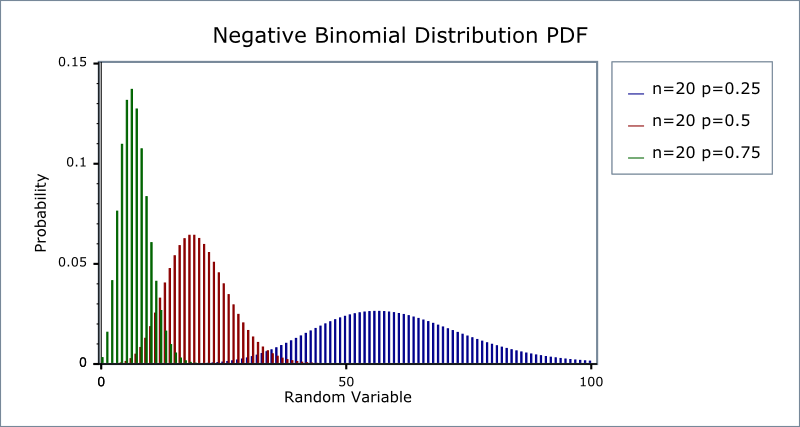
\includegraphics[width = 6 cm]{plots/part1/binomial.png}
		\end{figure}
		
		\column{0.5\textwidth}
		
		\begin{itemize}
			\item Binomial distribution
		\end{itemize}
		
	\end{columns}

\end{frame}

% Probability in a nutshell
\begin{frame}
	
	\frametitle{Probability in a nutshell}
	\framesubtitle{Poisson distribution}
	
	\footnotesize
	
	\begin{columns}	
		
		\column{0.5\textwidth}
		
		\begin{figure}
			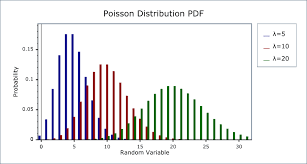
\includegraphics[width = 6 cm]{plots/part1/poisson.png}
		\end{figure}
		
		\column{0.5\textwidth}
		
		\begin{itemize}
			\item Poisson distribution
		\end{itemize}
		
	\end{columns}

\end{frame}

% Probability in a nutshell
\begin{frame}
	
	\frametitle{Probability in a nutshell}
	\framesubtitle{Continuous probability}

	\footnotesize

	Compute probability of measuring a particular height \\
	Used when comparing means

\end{frame}

% Probability in a nutshell
\begin{frame}

	\frametitle{Probability in a nutshell}
	\framesubtitle{Gaussian distribution}
	
	\footnotesize
	
	\begin{columns}	
	
		\column{0.5\textwidth}
		
		\begin{figure}
			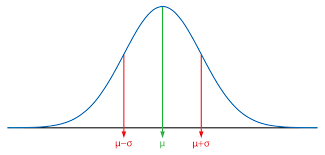
\includegraphics[width = 6 cm]{plots/part1/gaussian.png}
		\end{figure}
		
		\column{0.5\textwidth}
		
		\begin{itemize}
			\item Gaussian distribution
		\end{itemize}
		
	\end{columns}

\end{frame}

\begin{frame}
	
	\frametitle{Probability in a nutshell}
	\framesubtitle{Mean and variance}
	
	\footnotesize
	
	\begin{columns}	
		
		\column{0.5\textwidth}
		
		\begin{figure}
			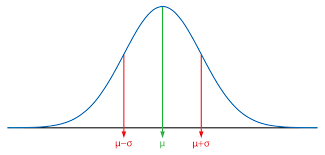
\includegraphics[width = 6 cm]{plots/part1/gaussian.png}
		\end{figure}
		
		\column{0.5\textwidth}
		
		\begin{itemize}
			\item Momenta of a distribution
			\item Mean, variance, skewness, kurtosis
		\end{itemize}
		
	\end{columns}

\end{frame}

% Probability in a nutshell
\begin{frame}
	
	\frametitle{Probability in a nutshell}
	\framesubtitle{Exercises in R}
	
	\footnotesize

	\href{https://lmsbioinformatics.github.io/LMS_StatisticsInR/course/CBW_StatisticsInR_course.html}{https://lmsbioinformatics.github.io/LMS\_StatisticsInR/course/CBW\_StatisticsInR\_course}

\end{frame}

%
% Linear models ..................................................................
%

% Linear models
\begin{frame}

	\center{\color{blue}Chapter II \\ Linear models}

\end{frame}

% Linear models
\begin{frame}

	\frametitle{Linear models}
	\framesubtitle{What is a linear model}

	\footnotesize
	
	\begin{columns}
		
		\column{0.5\textwidth}
		
		\begin{enumerate}
			\item Find a function that describes a set of observations
		\end{enumerate}
		
		\column{0.45\textwidth}
		
		\begin{figure}[!htb]
			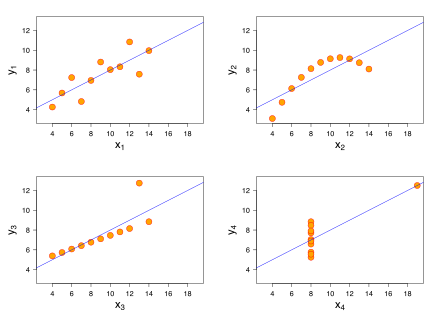
\includegraphics[width = \linewidth]{plots/part2/linear_model.png}
		\end{figure}
	
	\end{columns}

\end{frame}

% Linear models
\begin{frame}
	
	\frametitle{Linear models}
	\framesubtitle{Fitting a linear model}
	
	\footnotesize
	
	\begin{columns}
		
		\column{0.5\textwidth}
		
		\begin{enumerate}
			\item Fit a linear model
			\item Measuring differences - residuals
			\item Evaluate fit  - correlation coefficient
		\end{enumerate}
		
		\column{0.45\textwidth}
		
		\begin{figure}[!htb]
			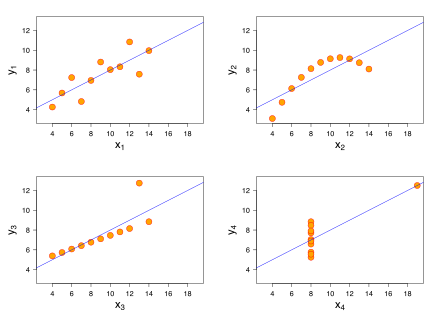
\includegraphics[width = \linewidth]{plots/part2/linear_model.png}
		\end{figure}
		
	\end{columns}

\end{frame}

% Linear models
\begin{frame}
	
	\frametitle{Linear models}
	\framesubtitle{Advanced topics}
	
	\footnotesize
	
	\begin{columns}
		
		\column{0.5\textwidth}
		
		\begin{enumerate}
			\item (...)
		\end{enumerate}
		
		\column{0.45\textwidth}
		
		\begin{figure}[!htb]
			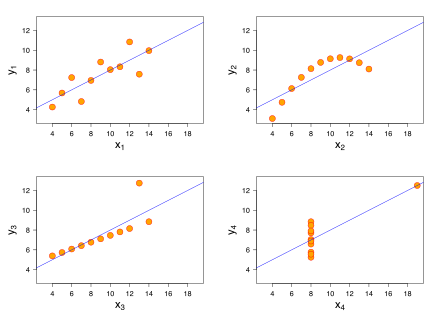
\includegraphics[width = \linewidth]{plots/part2/linear_model.png}
		\end{figure}
		
	\end{columns}

\end{frame}

% Linear models
\begin{frame}
	
	\frametitle{Linear models}
	\framesubtitle{Exercises in R}
	
	\footnotesize

	\href{https://lmsbioinformatics.github.io/LMS_StatisticsInR/course/CBW_StatisticsInR_course.html}{https://lmsbioinformatics.github.io/LMS\_StatisticsInR/course/CBW\_StatisticsInR\_course}


\end{frame}

%
% Hypothesis testing ..................................................................
%

% Hypothesis testing
\begin{frame}

	\center{\color{blue}Chapter III \\ Hypothesis testing}

\end{frame}

% Hypothesis testing
\begin{frame}
	
	\frametitle{Hypothesis testing}
	\framesubtitle{Introduction}
	
	\footnotesize
	
	\begin{itemize}
		\item Null hypothesis and alternative hypothesis
		\item Statistic tests and p-values
		\item $\chi^{2}$-test, $t$-test, Wald test
		\item Exercises in R
	\end{itemize}

\end{frame}

% Hypothesis testing
\begin{frame}
	
	\frametitle{Hypothesis testing}
	\framesubtitle{Compare different models}
	
	\footnotesize
	
	\begin{columns}
		
		\column{0.5\textwidth}
		
		\begin{enumerate}
		\item Null and alternative hypothesis
		\end{enumerate}
		
		\column{0.45\textwidth}
		
		\begin{figure}[!htb]
		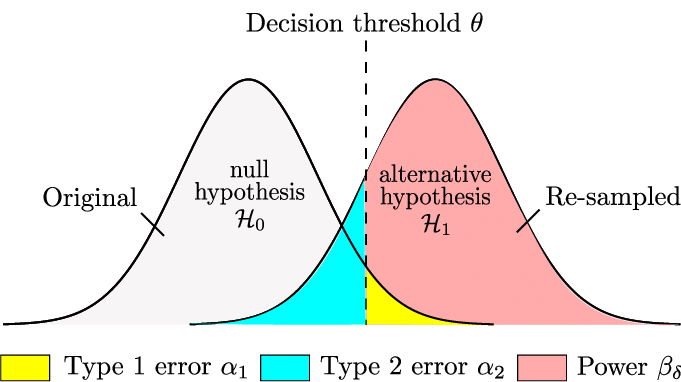
\includegraphics[width = \linewidth]{plots/part3/hypothesis.png}
		\end{figure}
	
	\end{columns}

\end{frame}

% Hypothesis testing
\begin{frame}
	
	\frametitle{Hypothesis testing}
	\framesubtitle{Statistic test}
	
	\footnotesize
	
	\begin{columns}
		
		\column{0.5\textwidth}
		
		\begin{enumerate}
			\item Quantify the significance of an observation
			\item Certainty when accepting / rejecting a hypothesis
		\end{enumerate}
		
		\column{0.45\textwidth}
		
		\begin{figure}[!htb]
		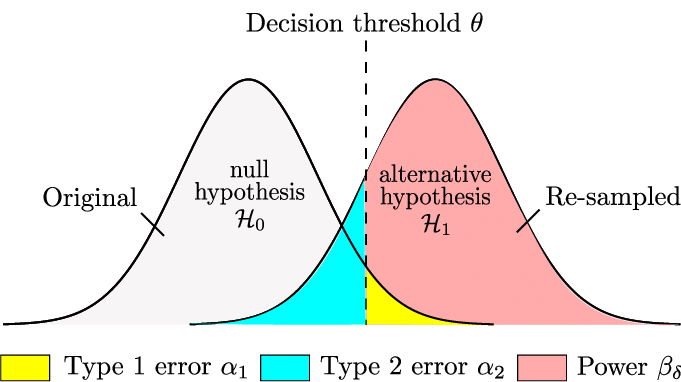
\includegraphics[width = \linewidth]{plots/part3/hypothesis.png}
		\end{figure}
	
	\end{columns}

\end{frame}

% Hypothesis testing
\begin{frame}
	
	\frametitle{Hypothesis testing}
	\framesubtitle{p-values}
	
	\footnotesize
	
	\begin{columns}
		
		\column{0.5\textwidth}
		
		\begin{enumerate}
			\item p-values
		\end{enumerate}
		
		\column{0.45\textwidth}
		
		\begin{figure}[!htb]
			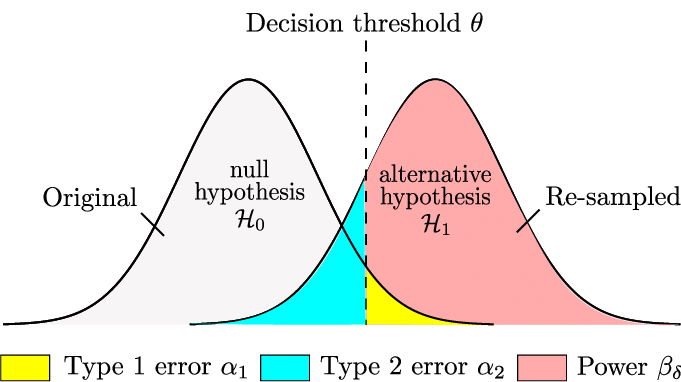
\includegraphics[width = \linewidth]{plots/part3/hypothesis.png}
		\end{figure}
		
	\end{columns}

\end{frame}

% Hypothesis testing
\begin{frame}
	
	\frametitle{Hypothesis testing}
	\framesubtitle{Exercises in R}
	
	\footnotesize
	
	\href{https://lmsbioinformatics.github.io/LMS_StatisticsInR/course/CBW_StatisticsInR_course.html\#/54}{https://lmsbioinformatics.github.io/LMS\_StatisticsInR/course/CBW\_StatisticsInR\_course}

\end{frame}

\end{document}